\begin{chapter}{Sample}
	\label{chapter:Sample}

	\sample is a tool for static analysis based on abstract interpretation that is currently being developed at \ethz. \sample is written completely in \scala. The project is open with respect to the choice of language as well as the type of analysis. The core of the \sample analyzer is split into two major packages which are both part of the \code{ch.ethz.inf.pm.sample} namespace. 

	\begin{itemize}
		\item The \code{abstractdomain} package contains classes representing the concepts related to abstract interpretation.
		\item The package \code{oorepresentation} contains the facilities related to analyzing an object oriented language.
	\end{itemize}

	I will start by discussing the former in Section \ref{section:abstractdomainrepresentation} before going into details about the specifics of object oriented languages in Section \ref{section:objectorientedrepresentation}. This is not meant to be a comprehensive documentation of the \sample project but rather a qualitative overview of the architecture providing the foundation for the coming chapters. Unfortunately, there is currently not much more documentation available and, since \sample is still under active development, the following material is a snapshot of the current development state. Furthermore, the active development also implies that there are features not yet implemented. The current limitations are briefly discussed in Section \ref{section:samplelimitations}.

	% ABSTRACT DOMAIN REPRESENTATION

	\begin{section}{Abstract Domain Representation}
		\label{section:abstractdomainrepresentation}

		The \code{abstractdomain} package is responsible for handling the abstract domains. A coarse overview of the package is given in Figure \ref{figure:abstractdomain}.
		
		\begin{figure}
			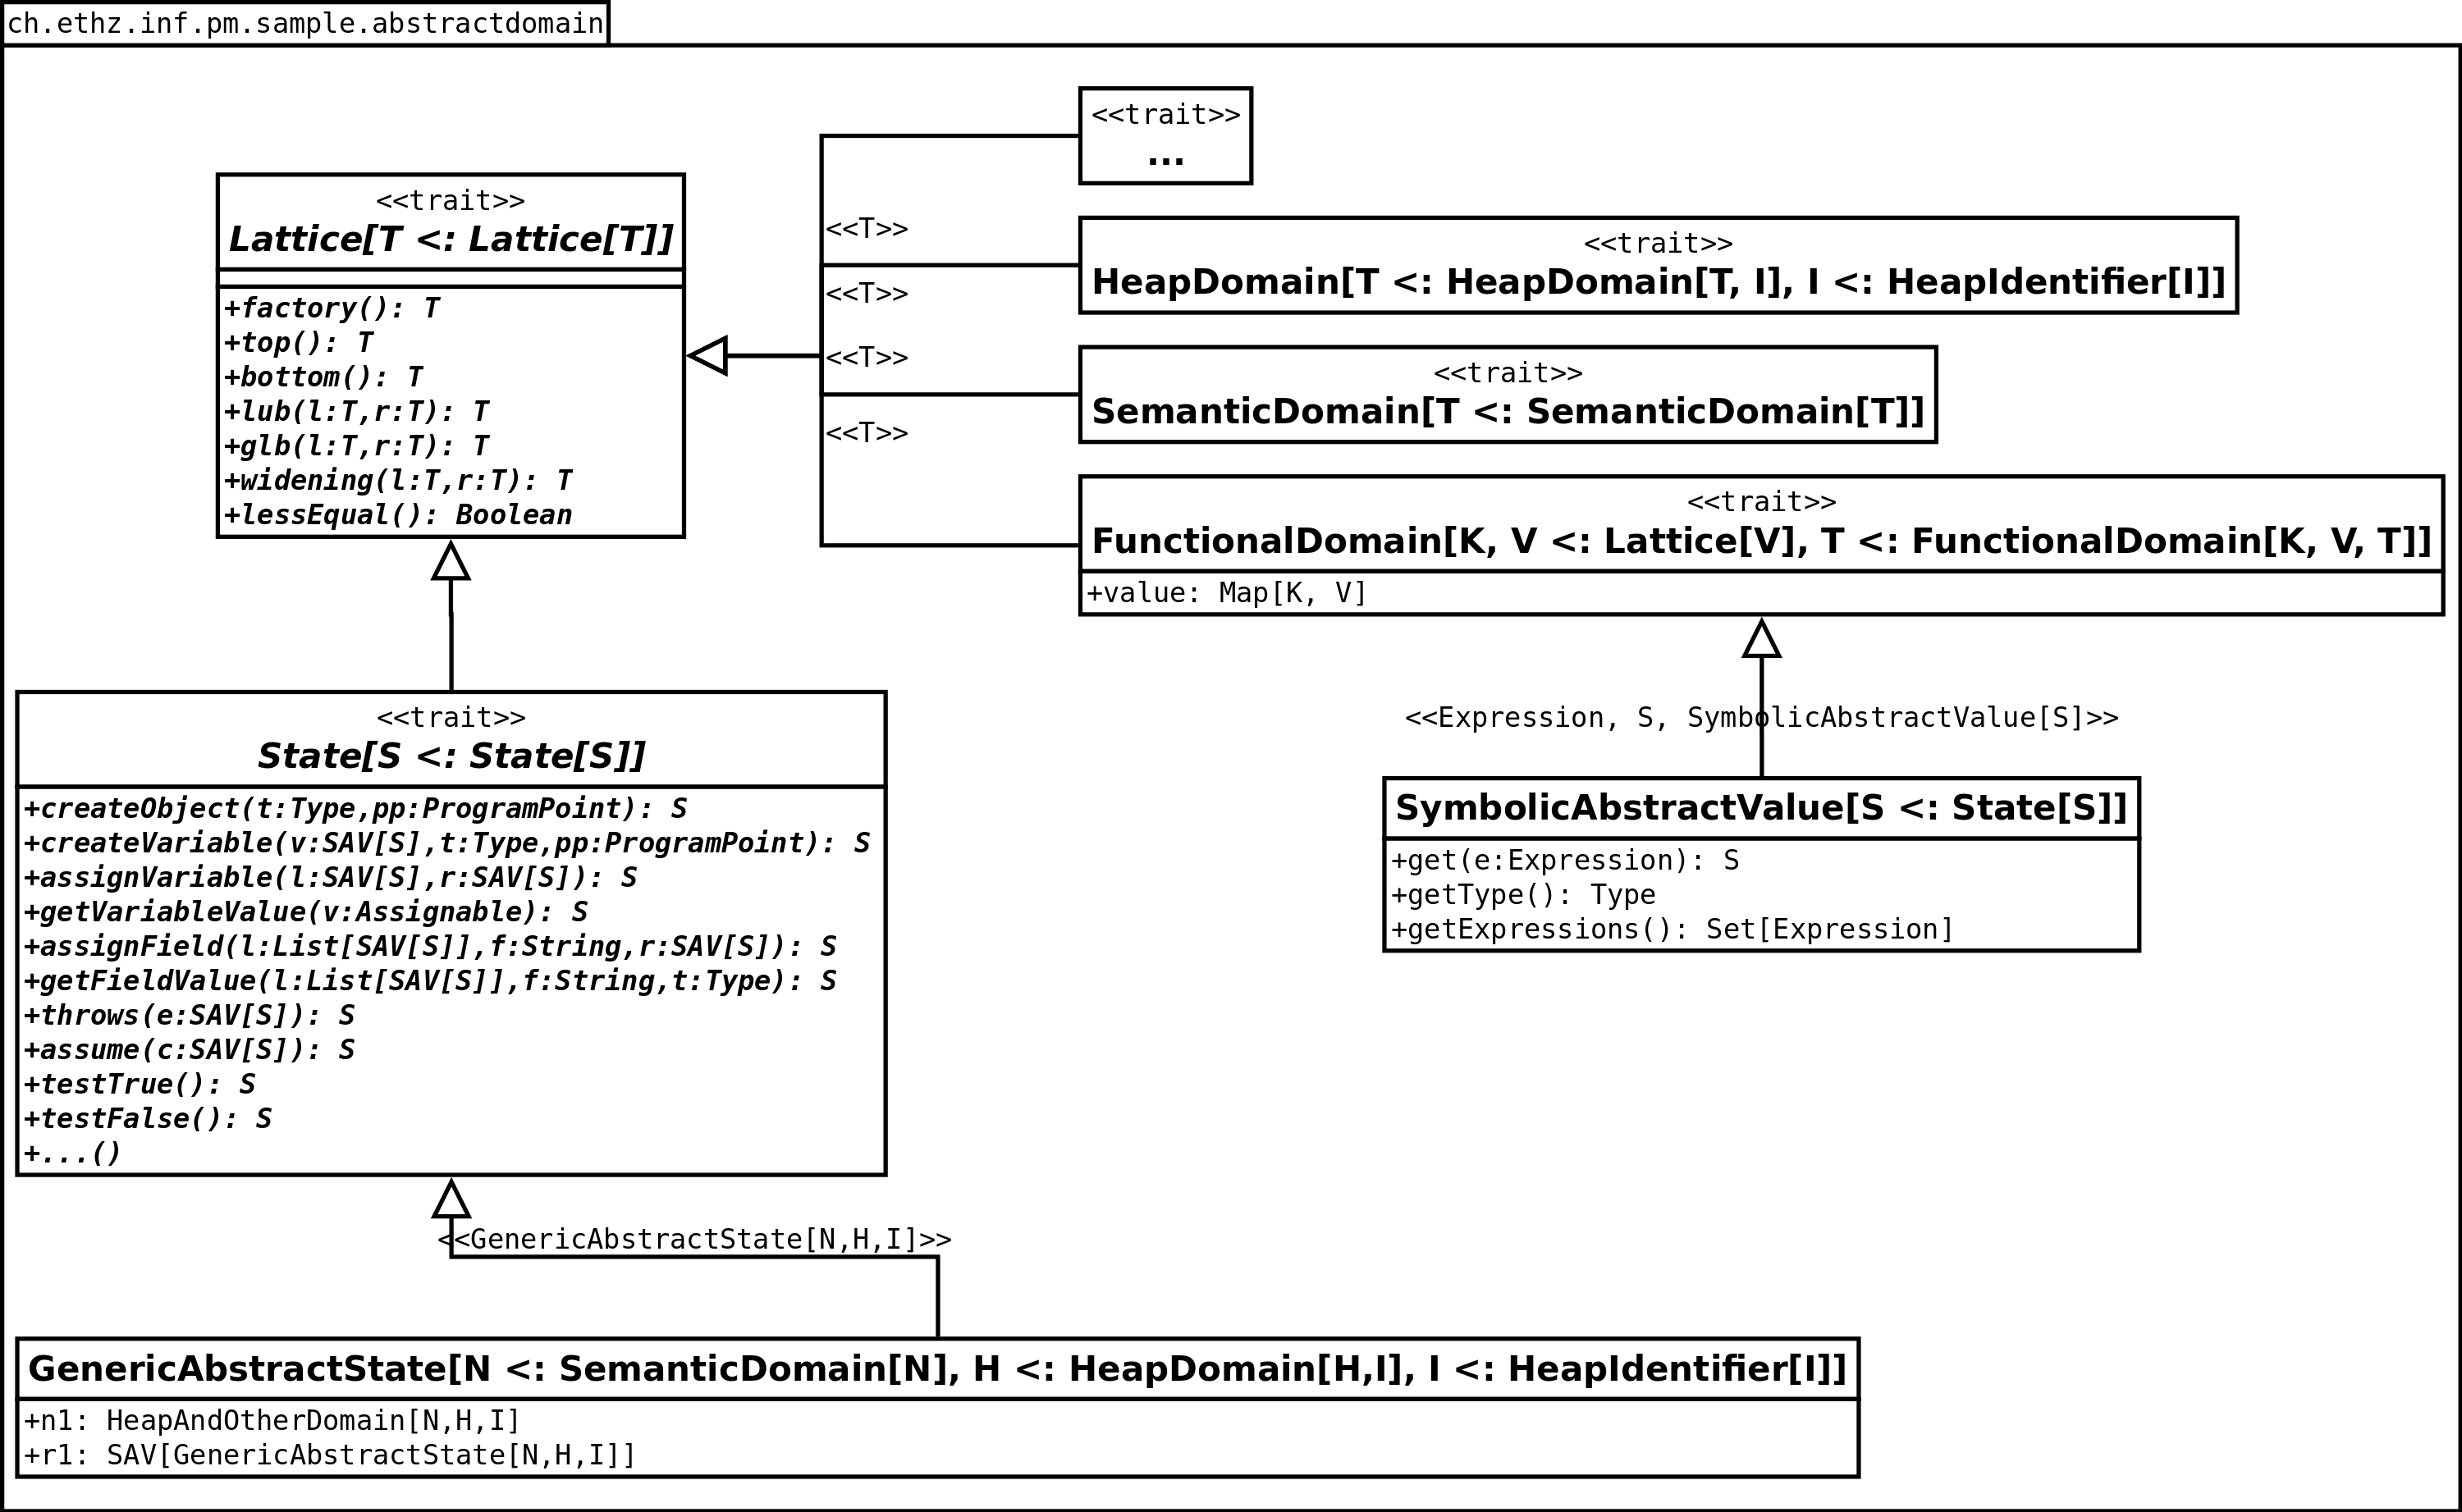
\includegraphics[width=\textwidth]{Diagrams/abstractdomain.png}
			\caption{The \code{abstractdomain} Package}
			\label{figure:abstractdomain}
		\end{figure}

		% LATTICE

		\begin{subsection}{Lattice}
			At the root of the inheritance tree is the \code{Lattice} trait which, as its name already suggests, represents a lattice as described in Section \ref{section:abstraction}. It provides factory methods for elements, the $\top$ as well as the $\bot$ element (\code{factory}, \code{top}, \code{bottom}). Furthermore, the \code{lub}, \code{glb} and \code{widening} compute the least upper bound, the greatest lower bound and the widening of two elements respectively. Most importantly, implementing classes have to provide an implementation for the ordering relation (\code{lessEqual}). It is discussed first because of its widespread usage throughout \sample. There are few classes that do not incorporate or at least interact with this trait.
		\end{subsection}

		% VALUES

		\begin{subsection}{Values}
			The class \code{Expression}, which is not depicted in the figure, represents the result of a statement. This result can have several possible forms amongst others are constants, variables and arithmetic as well as boolean expressions. Although it is not commonly the case, values in \sample need not be generated deterministically and hence expressions are not sufficient to represent values during the analysis. \code{SymbolicAbstractValue} (abbreviated \code{SAV} in Figure \ref{figure:abstractdomain}) deals with this subtlety by relating expressions to the states they where generated in. A symbolic abstract value can therefore represent multiple values at once. The following example attempts to clarify this concept.

			\begin{example}
				\label{example:symbolicabstractvalue}
				Some languages such as \scala allow conditionals to return values. Consider the assignment \code{r = if (x < 0) -1 else 1}. Assuming that evaluating the numerical constant \code{-1} results in a state \code{p} and evaluating \code{1} results in the state \code{q} respectively, the value representation assigned to \code{r} will be of the form $\{\code{-1} \mapsto \code{p}, \ \code{1} \mapsto \code{q}\}$.
				\exampleend
			\end{example}
		\end{subsection}

		% STATES

		\begin{subsection}{States}
			The \code{State} trait is the most fundamental trait of the \sample project. It represents abstract states of the analysis. A state's behavior is specific to the kind of analysis that is performed and the implementing subclasses have to provide the details.

			These details include the basic abstract operations and define what happens when, for example, a variable is created (\code{createVariable}), when a variable is assigned some value (\code{assignVariable}) but also what happens when a variable is read (\code{getVariableValue}) etc.

			Furthermore, the state describes what happens when some expression is evaluated in the context of the current state (\code{assume}). A special case occurs when the current context is evaluated to \code{true} or \code{false} respectively (\code{testTrue}, \code{testFalse}). This is the mechanism that allows conditionals to be handled by the analysis. Depending on whether the analysis follows the \code{true}-branch or the \code{false}-branch during the analysis the branching condition is evaluated accordingly.
			All these operations have in common that they do not modify the state objects but result in new state objects representing the modified state after applying the corresponding operations.

			Since it should be possible to compare and combine states, the trait also incorporates the \code{Lattice} trait.

			% The Generic Abstract State

			\begin{subsubsection}{The Generic Abstract State}
				A default implementation of the \code{State} trait is provided by the \code{GenericAbstractState} class. This implementation combines two abstract domains. The first one is a domain that keeps track of the heap structure during the analysis. The second can be any other analysis that implements the \code{SemanticDomain} trait, a simplification of the \code{State} trait allowing subclasses to safely ignore heap related concepts.

				Apart from managing the two domains, the generic abstract state also keeps track of what expression has last been evaluated in the current state in form of the \code{SymbolicAbstractValue} \code{r1}. Keeping track of the current expression not only makes it simple to implement the previously discussed \code{testTrue}/\code{testFalse} methods, but also makes it possible to support the assignment of more complex statements (see Example \ref{example:symbolicabstractvalue}).
			\end{subsubsection}
		\end{subsection}
	\end{section}

	% OBJECT ORIENTED REPRESENTATION

	\begin{section}{Object Oriented Representation}
		\label{section:objectorientedrepresentation}

		The other important package \code{oorepresentation} is roughly depicted in Figure \ref{figure:oorepresentation}. Its main responsibilities are the handling of some object oriented language, this includes the handling of the fixed point iteration discussed in Section \ref{section:StaticAnalysis}.

		\begin{figure}
			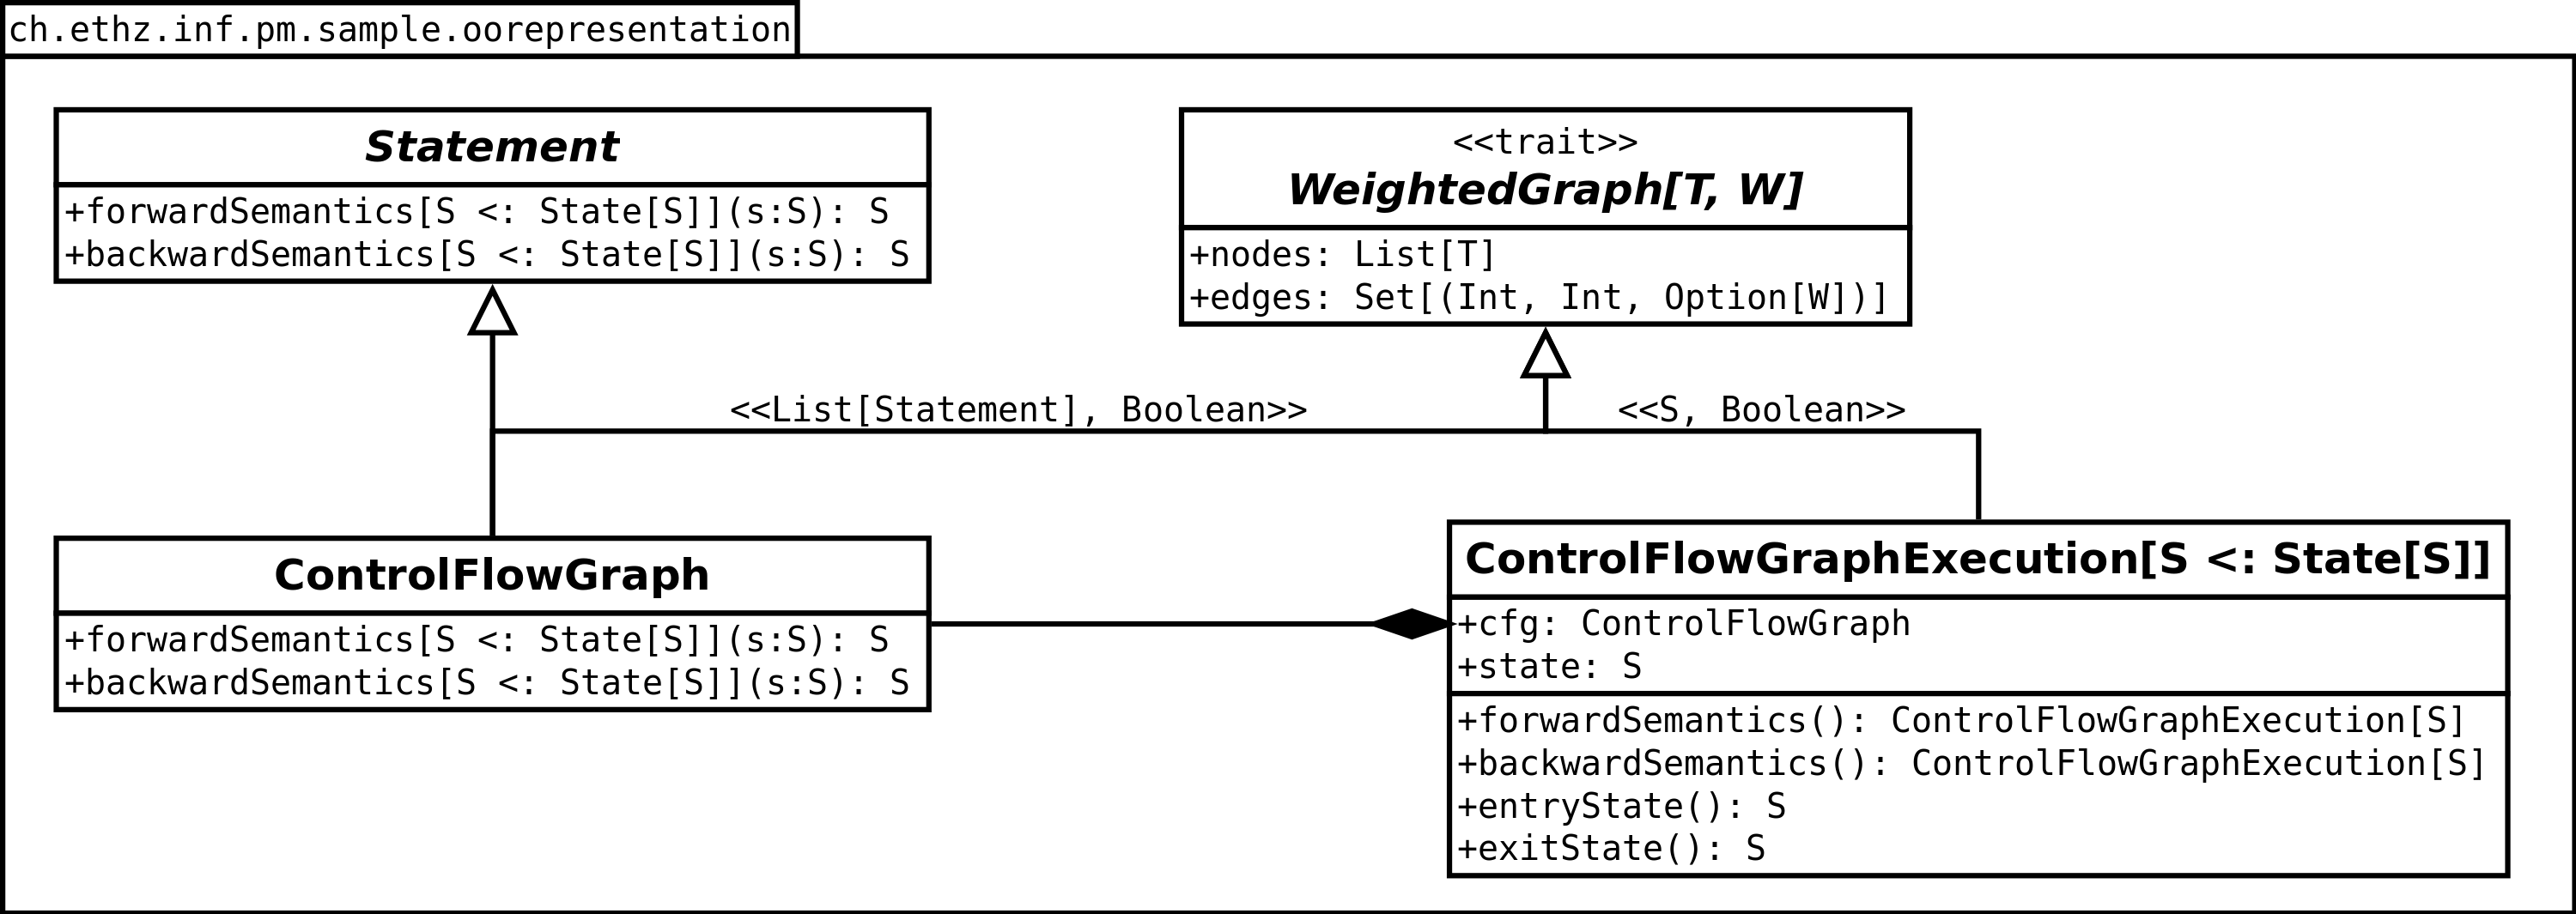
\includegraphics[width=\textwidth]{Diagrams/oorepresentation.png}
			\caption{The \code{oorepresentation} Package}
			\label{figure:oorepresentation}
		\end{figure}

		% CLASSES, METHODS AND STATEMENTS

		\begin{subsection}{Classes, Methods and Statements}
			Not listed in the figure are the classes representing the standard object oriented concepts. Classes are represented by \code{ClassDefinition} and provide access like most common introspection frameworks. The class definition provides access to its methods of type (\code{MethodDeclaration}) which in turn provide access to their execution body as \code{ControlFlowGraph} object. Instances of these classes are language specific and are generated from implementations of the \code{Compiler} trait. The \sample project currently provides compilers for \javabytecode and for \scala.

			The second basic notion not entirely depicted in Figure \ref{figure:oorepresentation} is that of a \code{Statement}. Case classes for assignments (\code{Assignment}), method calls (\code{MethodCall}) etc. provide implementations for this abstract class. A list of all subclasses is depicted in Figure \ref{figure:Statement}. These implementations of \code{Statement} mainly provide access to their semantics. The \code{forwardSemantics} (\code{backwardSemantics}) takes a state as argument and returns a state representing the analysis after (before) that statement is executed.

			\begin{figure}
				\centering
				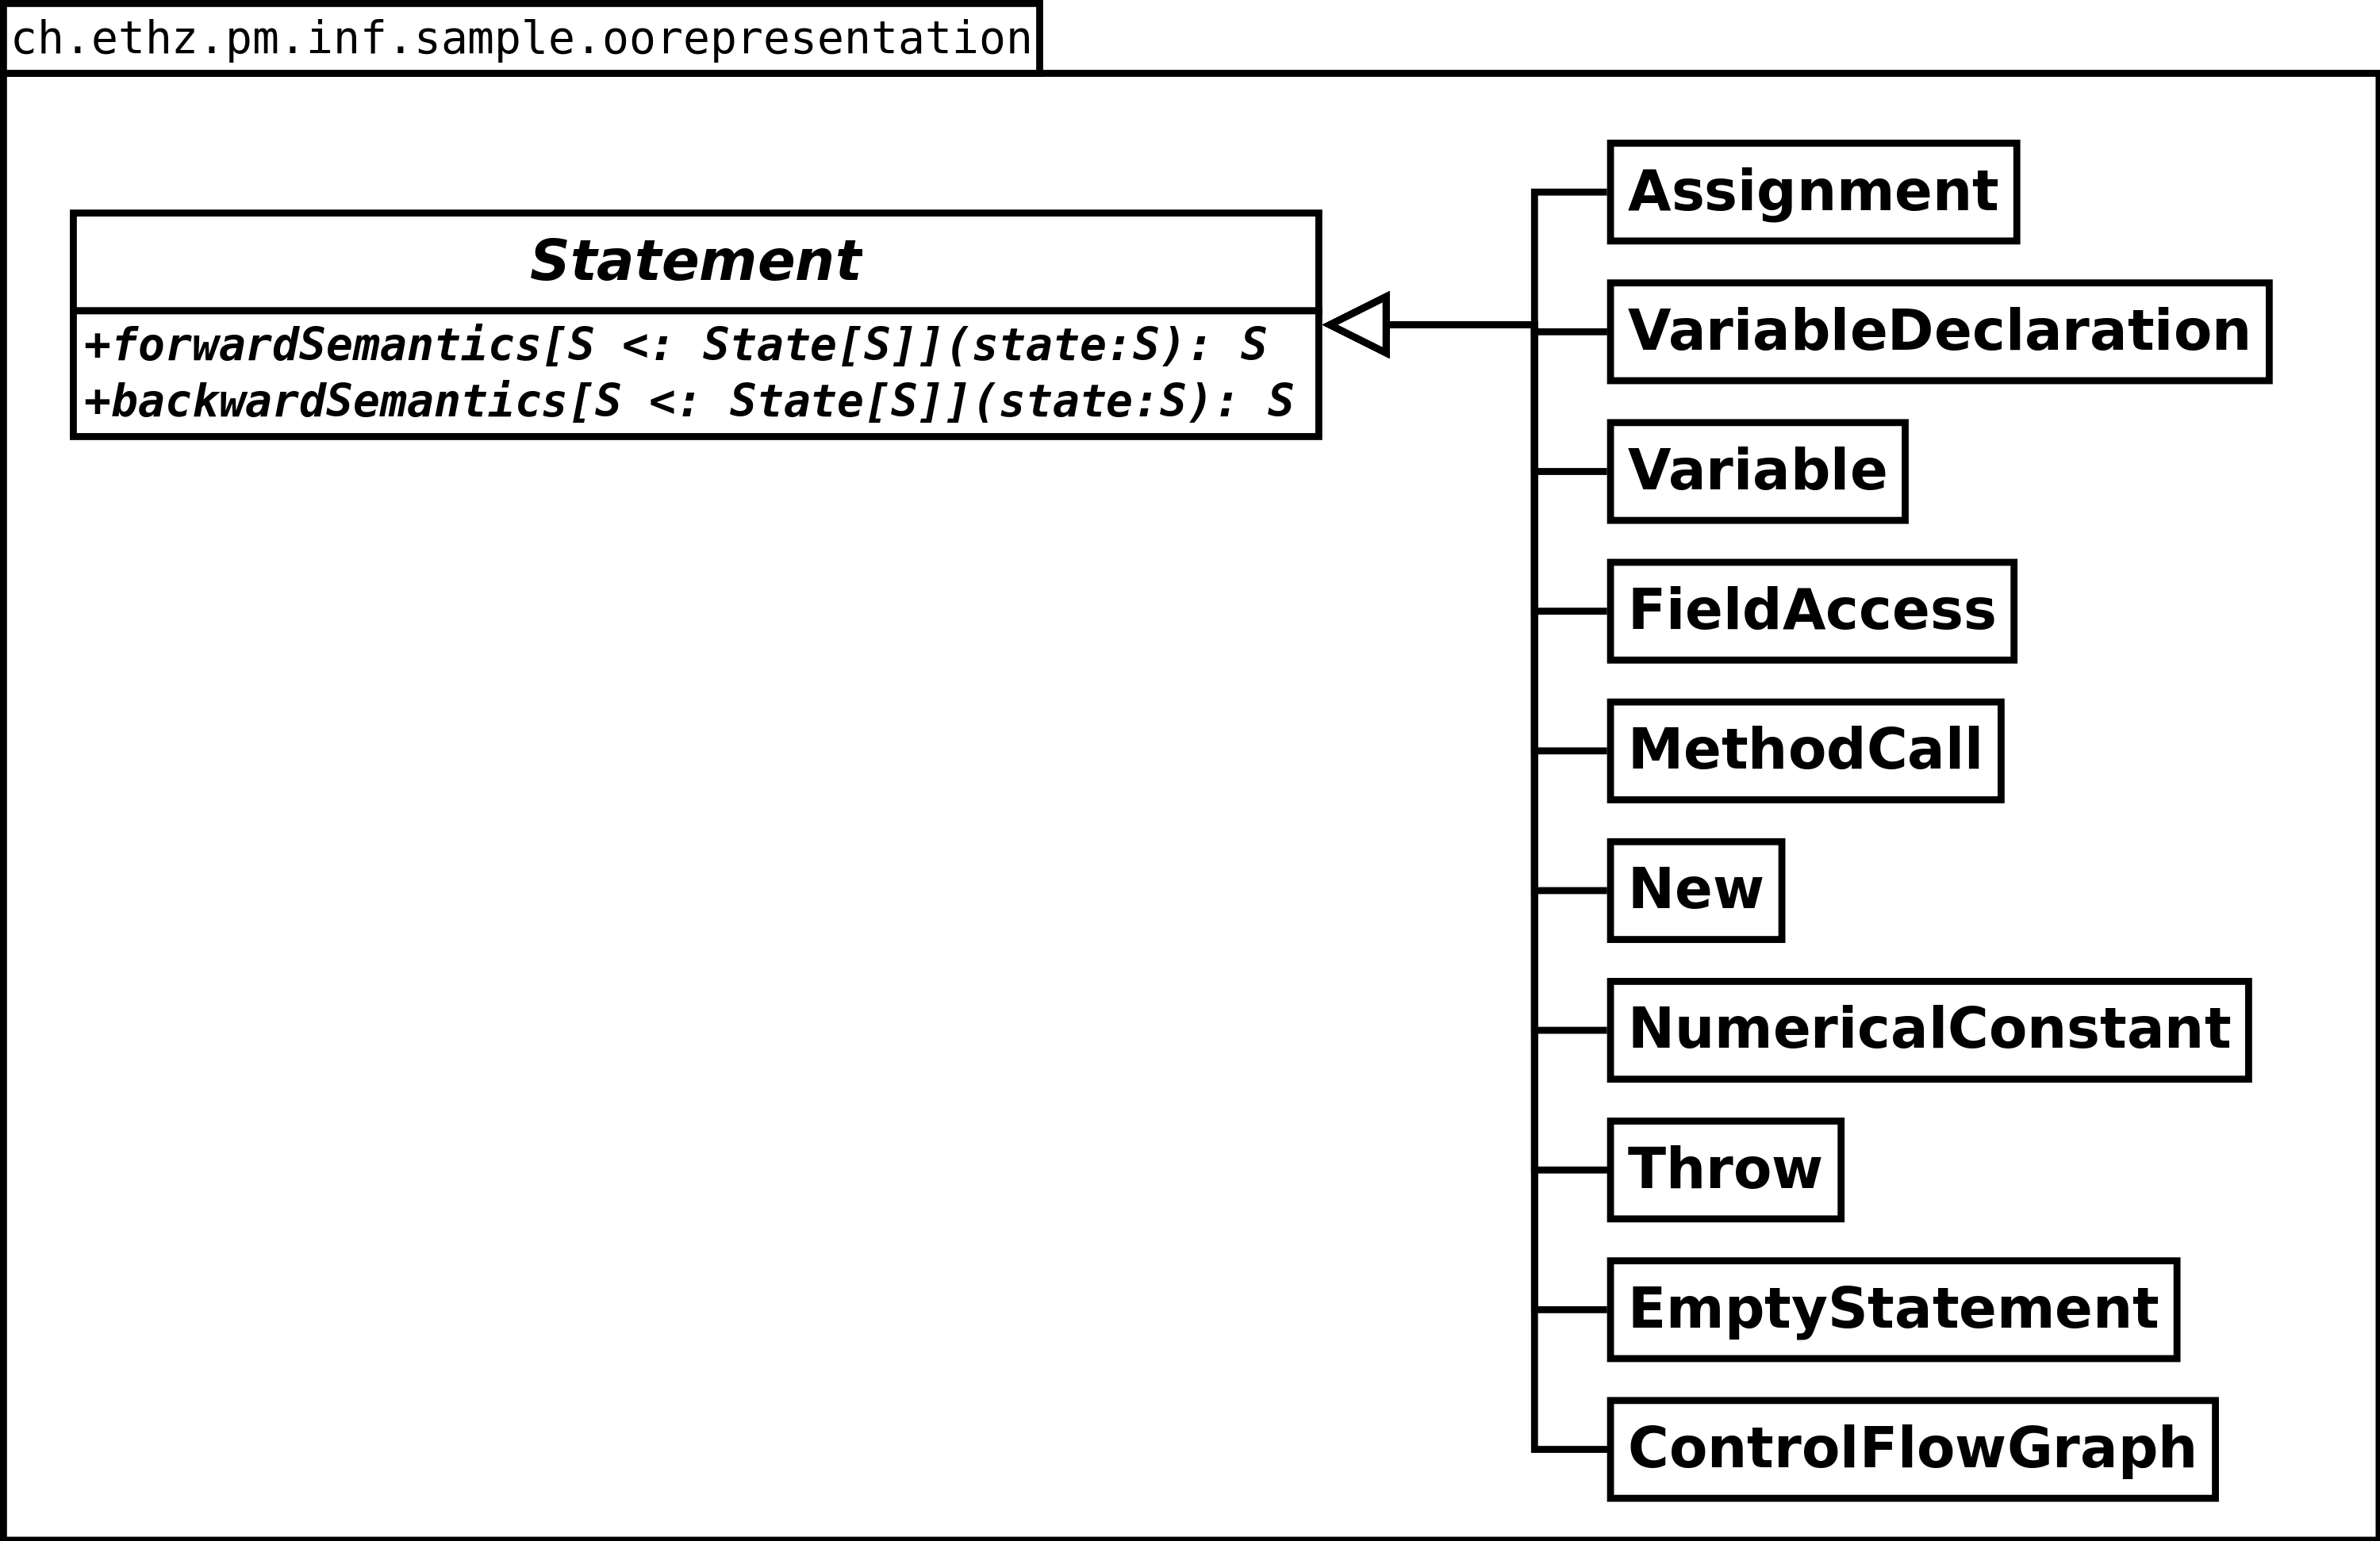
\includegraphics[width=0.7\textwidth]{Diagrams/Statement.png}
				\caption{The \code{Statement} Subclasses}
				\label{figure:Statement}
			\end{figure}

		\end{subsection}

		% CONTROL FLOW GRAPH

		\begin{subsection}{Control Flow Graph}
			At the center of the package are two implementations of the \code{WeightedGraph} trait representing a generic graph with weighted edges. The trait takes two type parameters specifying the type of the node and the type of the weight of the edges. The first implementation is the \code{ControlFlowGraph} representing, the control flow graph of the method to be analyzed. The nodes contain lists of \code{Statement} objects and the edges may be weighted with optional \code{Boolean} values indicating conditional branches of the control flow. An example of such a control flow graph was presented earlier in Figure \ref{figure:positivecfg}.
		\end{subsection}

		% CONTROL FLOW GRAPH EXECUTION

		\begin{subsection}{Control Flow Graph Execution}
			The second type of weighted graph is \code{ControlFlowGraphExecution}. For a given control flow graph and a state, the execution of the control flow can also be represented as graph. Depending on the type of the analysis, the provided state denotes either the entry state (forward analysis) or the exit state (backward analysis) of the system. Then, for each node of the control flow graph containing $n$ statements, the corresponding node in the execution graph contains $n+1$ states. The state $i+1$ of the node then represents the state before statement $i+1$ and after statement $i$. The edge sets of two corresponding control flow and control flow execution graphs are identical.

			The actual computation of the states of the control flow execution is the subject of the next section.
		\end{subsection}

		% ANALYSIS

		\begin{subsection}{Analysis}
			The classes presented so far are already sufficient to perform static analyses. A client has to provide a control flow graph, which is usually acquired by compiling some source file and extracting the body of a method of a class. Furthermore, the initial state of the analysis has to be provided. This state is analysis specific but usually some kind of \code{GenericAbstractState} with a heap and some other domain. \sample includes various domains. Amongst those is an interface to \apron \cite{jeannet09}, a collection of common numerical domains. 

			% Fixed Point Iteration

			\begin{subsubsection}{Fixed Point Iteration}
				\label{subsection:FixedPointIteration}
				The method \code{forwardSemantics} of the \code{ControlFlowGraph} computes the exit state of the analysis for a given initial state. It works by returning the exit state of the \code{ControlFlowGraphExecution} generated by a call to \code{forwardSemantics} of the same class. This function in turn delegates the work to a private method called \code{semantics} which is the place where the fixed point iteration happens. The method takes as an argument a function performing a single iteration step and applies it until the states of the control flow graph execution do not change any more or until a widening limit is reached. The function used in the computation of the forward semantics is called \code{forwardSingleIteration} and is also a member of the \code{ControlFlowGraphExecution} class.

				This single iteration will be of importance for the discussion of some implementation details of the trace partitioning extension and will therefore be discussed in more detail. A single iteration steps over all nodes of the control flow graph. For each node it computes an entry state and stores it at position \code{0} in the corresponding execution graph node. The entry state is computed by a helper method (\code{entryState}) that collects, by means of the least upper bound, all last states of nodes in the execution graph that contain an edge pointing to the current node. If that edge is weighted by a \code{Boolean} value the corresponding state transformation, \code{testTrue} or \code{testFalse}, is applied beforehand.

				The missing states of the execution graph node are then computed by the \code{forwardBlockSemantics}. This method subsequently computes the forward semantics of each statement of the control flow graph block, starting with the previously computed entry state and stores the result in the next element of the execution graph list.
			\end{subsubsection}

			% Parameters

			\begin{subsubsection}{Parameters}
				The singleton \code{SystemParameters} specifies various details of the analysis. Most notably, it defines the widening limit (\code{wideningLimit}) that specifies when the fixed point iteration switches from using the least upper bound to applying the widening, thereby forcing the iteration to converge. 
				
				The system parameters also specify the property of interest for the analysis. Properties are of type \code{Property} and define a method that is automatically passed the final control flow graph execution of the analysis. \sample already defines a few properties, such as the \code{DivisionByZero} property that generates a warning message if there is a possible division by zero.

				During the analysis, the parameters singleton keeps track of what class, method etc. is being analyzed at the moment. Furthermore, specifying different output objects (\code{progressOutput}, \code{screenOutput}) allows the client to intercept and handle the text output of the static analyzer.
			\end{subsubsection}
		\end{subsection}
	\end{section}

	% LIMITATIONS

	\begin{section}{Limitations}
		\label{section:samplelimitations}

		As already hinted at, \sample is still under active development. This also means that there are currently several limitations as to what can be analyzed.

		There are some limitations as to what language constructs are supported in \sample. Interprocedural calls will be supported by the use of contracts. However, the contracts specification language is still under discussion and development. This is especially problematic for languages where native array access is modelled as a method call, which is the case in \scala. The problem can be addressed though by ``simulating'' arrays as will be seen later in this presentation.
		
		Furthermore, not all abstract domain implementations have fully matured yet. Most of the shortcomings are concerned with not fully implementing logic rules such as DeMorgan for negated boolean expressions or detecting contradictions in the internal state. While the former usually just ends the analysis with an exception, the latter can be problematic since it may result in states that are $\bot$ but are not recognized as such.
	\end{section}
\end{chapter}
